\newpage
\subsubsection{globale und lokale Extreme}

\begin{itemize}
    \item \textcolor{red}{${a,b}$ sind Randextreme}
    \item \textcolor{violet}{$x_1,x_2$ sind lokale Extreme}
\end{itemize}

\hfill \break
\begin{itemize}
    \item Globale Extrmes sind Extreme bezüglich des Gesammten Definitionsbereich.
    \item Lobale Extrmes sind Extreme bezüglich eines klienen Bereiches.
    \item Extremstellen haben wagrechte Tangenten mit der Steigung $0$
\end{itemize}

\hfill \break
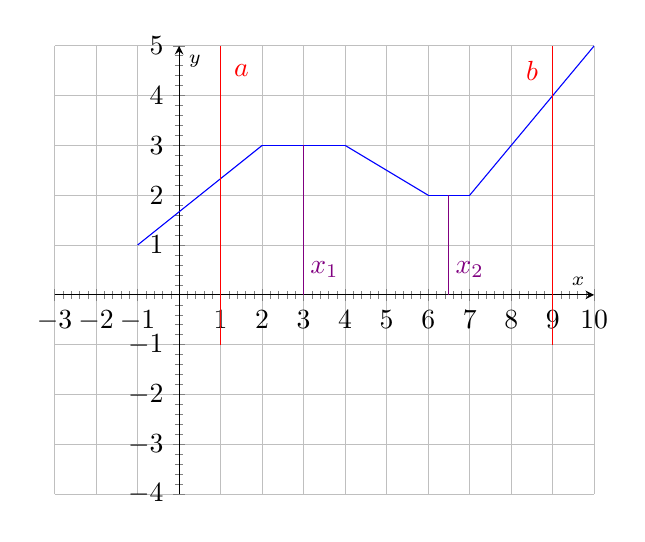
\begin{tikzpicture}[scale=1.0]
    \begin{axis}%
        [
            grid=major,
            xtick={-7,-6,...,11},
            minor x tick num=4, % 4 minor ticks => 5 subintervals
            xmin=-3,
            xmax=10,
            xlabel={\scriptsize $x$},
            axis x line=middle,
            ytick={-6,-5,...,6},
            minor y tick num=4,  % 4 minor ticks => 5 subintervals
            ymin=-4,
            ymax=5,
            ylabel={\scriptsize $y$},
            axis y line=middle,
            no markers,
            samples=100,
            domain=-6:6,
        ]
        \draw[blue] (-1,1) -- (2,3);
        \draw[blue] (2,3) -- (4,3);
        \draw[blue] (4,3) -- (6,2);
        \draw[blue] (6,2) -- (7,2);
        \draw[blue] (7,2) -- (10,5);
        \draw[red] (1,-1) -- (1,5);
        \draw[red] (9,-1) -- (9,5);
        \node[red] at (1.5,4.5) {$a$};
        \node[red] at (8.5,4.5) {$b$};

        \draw[violet] (3,0) -- (3,3);
        \draw[violet] (6.5,0) -- (6.5,2);
        \node[violet] at (3.5,0.5) {$x_1$};
        \node[violet] at (7,0.5) {$x_2$};
    \end{axis}
\end{tikzpicture}